\documentclass{article}

%%% Fill details here (in the second brackets)
\newcommand{\name}{Weijie Gan}     % Your name (First Last)
\newcommand{\wustlkey}{gan.weijie}             % Your WUSTL Key
%%%

%%%%%%%%%%%%%%%%%%%%%% Formatting Stuff %%%%%%%%%%%%%%%%%%%%%%%%%%%
\usepackage{times}
\usepackage[T1]{fontenc}
 
\setlength{\parskip}{1em}\setlength{\parindent}{0pt}
\linespread{1.25}
\usepackage[margin=0.7in,top=1in]{geometry}\usepackage{fancyhdr}
\pagestyle{fancy}\lhead{\bf \name}\rhead{\bf \wustlkey}\cfoot{\thepage}
\newcommand{\info}{\clearpage \subsection*{Information}}
\newcommand{\solution}[1]{\clearpage \subsection*{Solution #1}}
\newcommand{\spart}[1]{\paragraph{(#1)}}
%%%%%%%%%%%%%%%%%%%%%%%%%%%%%%%%%%%%%%%%%%%%%%%%%%%%%%%%%%%%%%%%%%%

%%% Add any more packages if you want to
\usepackage{amsmath,graphicx}

\begin{document}
%%%%% Main Body goes here

% Begin solution to every problem like this.
\solution{1}
\spart{a}
Since there are $J$ outliers and total $N$ correspondences, amount of inliers is $N-J$.
And because $K$ points are selected randomly from all $N$ correspondences, the possibility is:
Especially, $C(n, k)$ means all choice when we select disordered $k$ samples within $n$ data.
$$
  \begin{aligned}
    P_1 & = \frac{C(N-J, K)}{C(N, K)} \\
    & = \frac{\frac{(N-J)!}{K!(N-J-K)!}}{\frac{N!}{K!(N-K)!}} \\
    & = \frac{(N-J)!(N-K)!)}{N!(N-J-K)!} \\
  \end{aligned}
$$

\spart{b}
It's equivalent between $at\ least\ once$ with contrary of $None$. The result is:
$$
  \begin{aligned}
    P & = 1 - P(All\ K\ Points\ are\ outliers) \\
    P & =  1 - {(1 - P_1)}^T \\
    T\times In(1 - P_1) & = In(1-P) \\
    T & = \frac{In(1-P)}{In(1-P_1)} \\
    T & = \frac{In(1-P)}{In(1-\frac{(N-J)!(N-K)!}{N!(N-J-K)!})} \\
  \end{aligned}
$$ 
\spart{c}
Total amount of correspondences and inliers points are same with above problem. And all possible combination are still $C(K, N)$.
The correct combination is sum of $K$ samples in $I_1$ area, which means $C(I_1, K)$ and $K$ samples in $I_2$ area, which means $C(I_2, K)$. So, the result is:
$$
  \begin{aligned}
    P_3 & = \frac{C(I_1, K) + C(I_2, K)}{C(N, K)} \\
    P_3 & = \frac{\frac{I_1!}{K!(I_1-k)!} + \frac{I_2!}{K!(I_2-k)!}}{\frac{N!}{K!(N-K)!}} \\
  \end{aligned}
$$

\solution{2} 
\spart{a}
Code Output:
(Top Left) No outliers, simple fit Error = 0.00. 
(Top Right) 10pc outliers, simple fit Error = 0.41. 
(Bottom Left) 10pc outliers, 10 iters fit Error = 0.01. 
(Bottom Right) 50pc outliers, 10 iters fit Error = 1.26. 

The output figure is shown as figure [\ref{fig:prob2a}]. 
The choice when $outliers$ = 10$pc$ and $iters$ = 1, have the least fit error, since it has no outliers.
When $outliers$ = 10$pc$ and $iters$ = 1, fit error is large since some outliers point affect its first estimation.
If we drop all outliers point, fit error become acceptable as shown in choice when $outliers$ = 10$pc$ and $iters$ = 10.
The finial choice when $outliers$ = 100$pc$ and $iters$ = 10, isn' t good enough, since too many outliers have a really negative effective on its first estimation.
The first estimation leaves the true fit line too far. Drop some outliers based on the first estimation can not lead it return to the right fit line.

\begin{figure}[htbp]
  \centering
  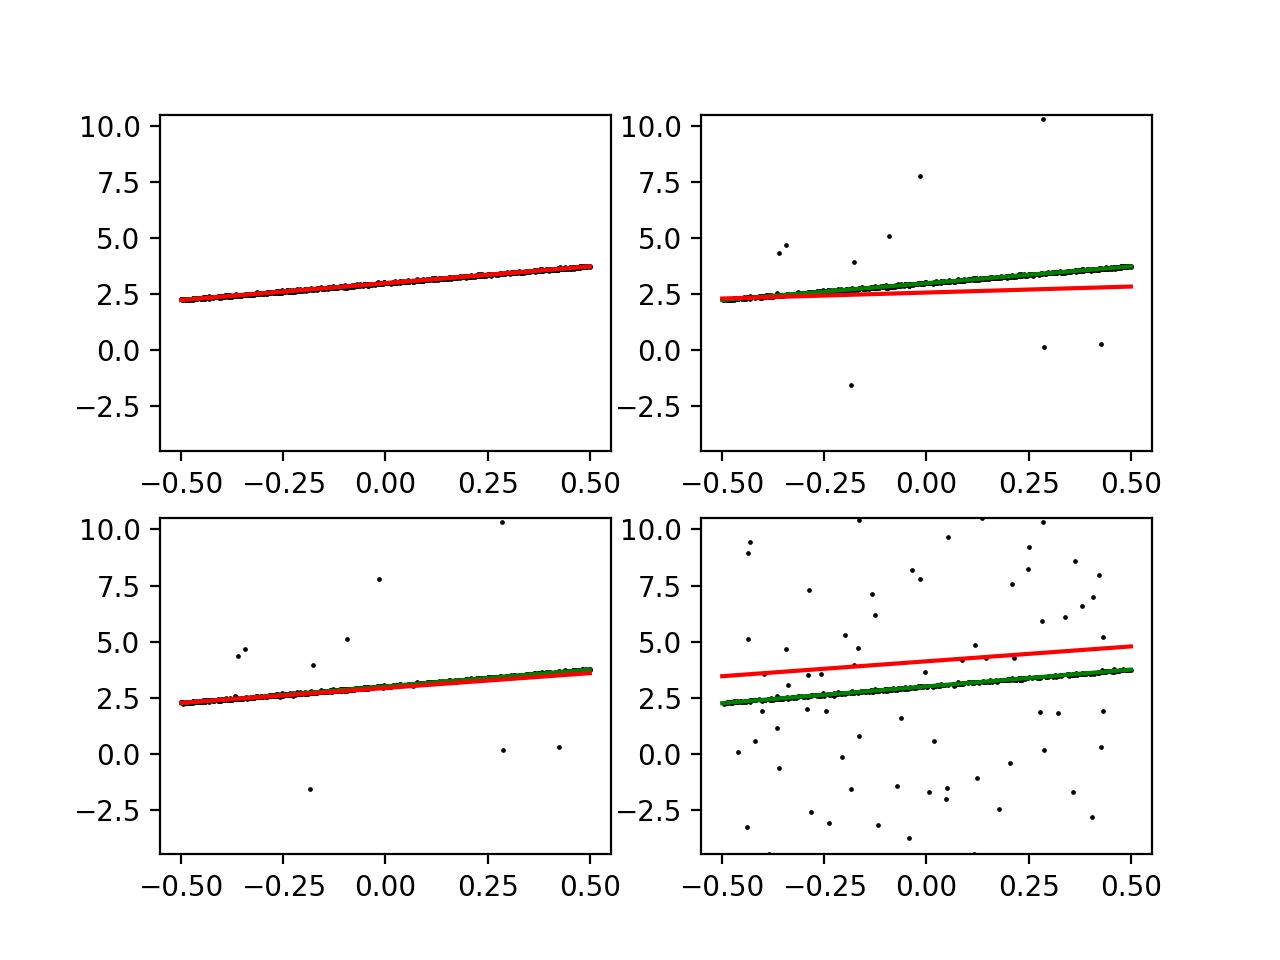
\includegraphics[height = 30em]{./code/outputs/prob2a.png}
  \caption{Output Figure in Prob2a}
  \label{fig:prob2a}
\end{figure}

\spart{b} I call the script 10 times. The result is shown as table [\ref{table:prob2b}]. 
Since mean and variation are all the least, the choice when $K$ = 5 and $N$ = 1000, returns the best fit most consistently.

The output figure is shown as figure [\ref{fig:prob2b}].
\begin{table}[htbp]
  \centering
  \begin{tabular}{|l|c|c|c|c|}
  \hline
  Count     & K = 50, N = 4, Error = & K = 5, N = 40, Error = & K = 50, N = 100, Error = & K = 5, N = 1000, Error = \\ \hline
  1         & 3.92                    & 32.64                   & 13.95                   & 0.19                    \\ \hline
  2         & 4                       & 2.32                    & 30.36                   & 0.19                    \\ \hline
  3         & 2.61                    & 0.3                     & 0.84                    & 1.13                    \\ \hline
  4         & 29.81                   & 0.98                    & 2.08                    & 0.64                    \\ \hline
  5         & 66.61                   & 0.85                    & 8.91                    & 0.16                    \\ \hline
  6         & 79.83                   & 3.34                    & 1.25                    & 1.15                    \\ \hline
  7         & 52.13                   & 1.56                    & 0.71                    & 0.89                    \\ \hline
  8         & 84.46                   & 0.33                    & 7.88                    & 4.55                    \\ \hline
  9         & 5.26                    & 1.05                    & 14.98                   & 0.27                    \\ \hline
  10        & 125.08                  & 6.37                    & 3.03                    & 0.2                     \\ \hline
  Mean      & 45.371                  & 4.974                   & 8.399                   & 0.937                   \\ \hline
  Variation & 1852.773            & 97.832            & 88.118       & 1.770            \\ \hline
  \end{tabular}
  \caption{Output Table in Prob2b}
  \label{table:prob2b}
\end{table}

\begin{figure}[htbp]
  \centering
  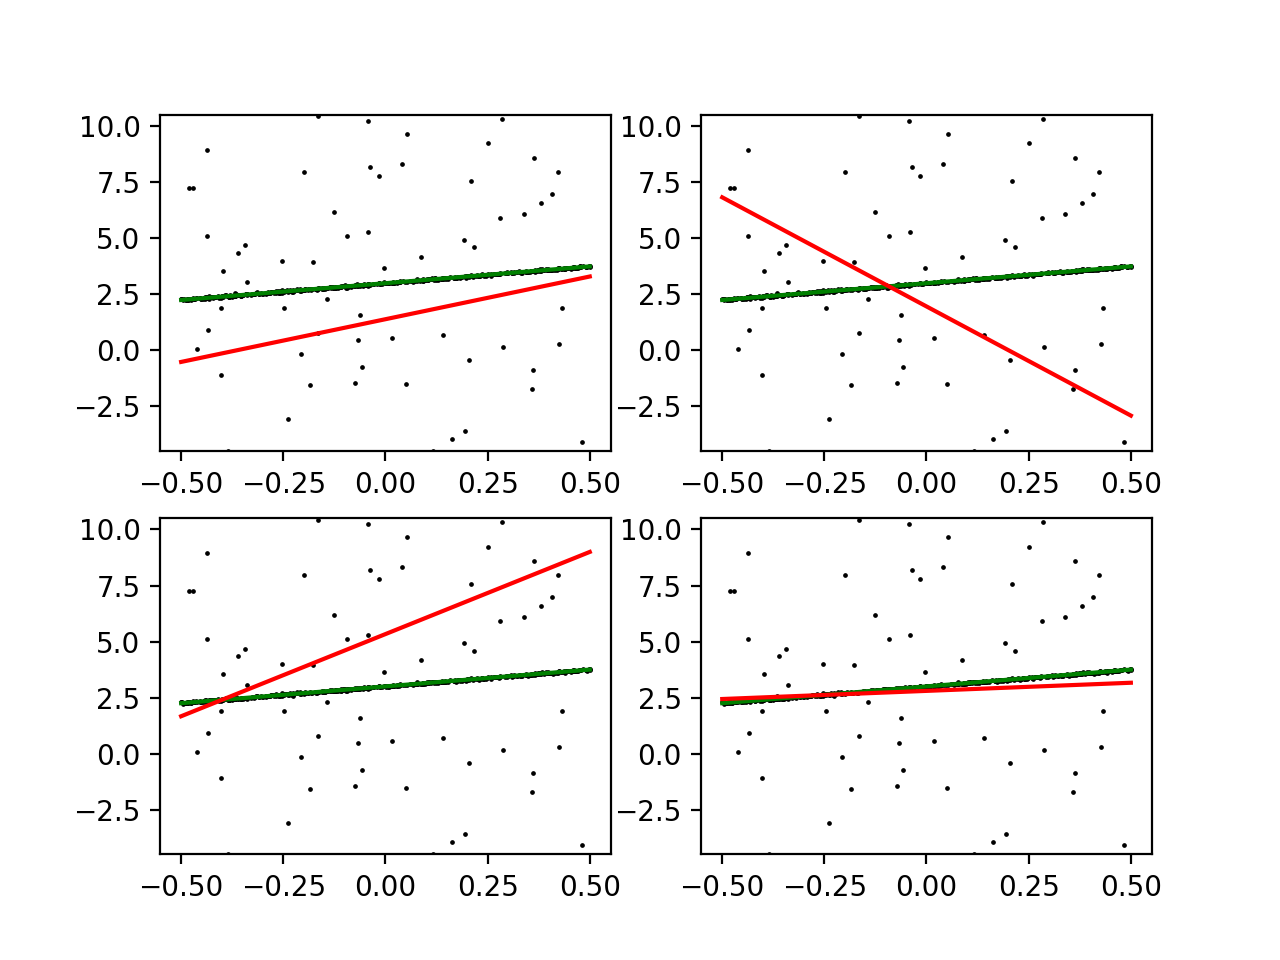
\includegraphics[height = 30em]{./code/outputs/prob2b.png}
  \caption{Output Figure in Prob2b}
  \label{fig:prob2b}
\end{figure}

\solution{3}
\spart{a}
Since there is no rotation and translation, matrix $[R|t]$ is same for 2 camera and we can ignore it in both camera 1 and camera 2.
So,
$$
  p^{(1)} = [K_1 0]p' = \begin{bmatrix}
    f_1 & 0 & W/2 & 0 \\
    0 & f_1 & H/2 & 0 \\
    0 & 0 & 1 & 0 \\
  \end{bmatrix}p'
$$
and 
$$
  p^{(2)} = [K_2 0]p' = \begin{bmatrix}
    f_2 & 0 & W/2 & 0\\
    0 & f_2 & H/2 & 0 \\
    0 & 0 & 1 & 0 \\
  \end{bmatrix}p'
$$
Suppose $p' = {[p'_1, p'_2, p_3', 1]}^T$, then
$$
  p^{(1)} = [K_1 0]p' = \begin{bmatrix}
    f_1 & 0 & W/2 & 0 \\
    0 & f_1 & H/2 & 0 \\
    0 & 0 & 1 & 0 \\
  \end{bmatrix}\begin{bmatrix}
    p'_1 \\
    p'_2 \\
    p'_3 \\
    1 \\
  \end{bmatrix} = \begin{bmatrix}
    f_1p'_1 + \frac{W}{2}p'_3 \\
    f_1p'_2 + \frac{H}{2}p'_3 \\
    p'_3 \\
  \end{bmatrix} = p'_3\begin{bmatrix}
    f_1\frac{p'_1}{p'_3} + \frac{W}{2} \\
    f_1\frac{p'_2}{p'_3} + \frac{H}{2} \\
    1 \\
  \end{bmatrix} 
$$
and
$$
  p^{(2)} = [K_2 0]p' = \begin{bmatrix}
    f_2 & 0 & W/2 & 0 \\
    0 & f_2 & H/2 & 0 \\
    0 & 0 & 1 & 0 \\
  \end{bmatrix}\begin{bmatrix}
    p'_1 \\
    p'_2 \\
    p'_3 \\
    1 \\
  \end{bmatrix} = \begin{bmatrix}
    f_2p'_1 + \frac{W}{2}p'_3 \\
    f_2p'_2 + \frac{H}{2}p'_3 \\
    p'_3 \\
  \end{bmatrix} = p'_3\begin{bmatrix}
    f_2\frac{p'_1}{p'_3} + \frac{W}{2} \\
    f_2\frac{p'_2}{p'_3} + \frac{H}{2} \\
    1 \\
  \end{bmatrix} 
$$

Because $p^{(1)}_1 = f_1\frac{p'_1}{p'_3} + \frac{W}{2}$ and $p^{(2)}_1 = f_2\frac{p'_1}{p'_3} + \frac{W}{2}$,
let $p^{(1)}_1 - p^{(2)}_1$:
$$
\begin{aligned}
  p^{(1)}_1 - p^{(2)}_1 & = (f_1 - f_2)\frac{p'_1}{p'_3} \\
  \frac{p'_1}{p'_3} & = \frac{p^{(1)}_1 - p^{(2)_1}}{f_1 - f_2} \\
\end{aligned}
$$
So, $p^{(1)}_1 = f_1\frac{p'_1}{p'_3} + \frac{W}{2} = f_1\frac{p^{(1)}_1 - p^{(2)}_1}{f_1 - f_2} + \frac{W}{2}$ and 
$$
  p^{(1)}_1 =  \frac{f_1}{f_2} p^{(2)}_1 - \frac{1}{2}(\frac{f_1}{f_2}-1)W
$$

Similarly, $p^{(1)}_2 =  \frac{f_1}{f_2} p^{(2)}_2 - \frac{1}{2}(\frac{f_1}{f_2}-1)H$.

\spart{b}
Suppose two cameras relate with same rotation matrix $R$ and translation matrix $t$, and extrinsic matrices are $K_1$ and $K_2$. 
Consider a plane in world 3D co-ordinate $p' = (p'_1, p'_2, 0, 1)$, projected plane $p^{(1)}$ in camera 1 is:
$$
  p^{(1)} = K_1 [R|t] p' = K_1 \begin{bmatrix}
    R_{11} & R_{12} & R_{13} & t_1 \\
    R_{21} & R_{22} & R_{23} & t_2 \\
    R_{31} & R_{32} & R_{33} & t_3 \\
  \end{bmatrix} {[p'_1, p'_2, 0, 1]}^T = K_1 \begin{bmatrix}
    R_{11}p'_1 + R_{12}p'_2 + t_1 \\
    R_{21}p'_1 + R_{22}p'_2 + t_2 \\
    R_{31}p'_1 + R_{32}p'_2 + t_3 \\
  \end{bmatrix}
$$

Similarly, projected plane $p^{(2)}$ in camera 1 is $p^{(2)} = K_2 \begin{bmatrix}
  R_{11}p'_1 + R_{12}p'_2 + t_1 \\
  R_{21}p'_1 + R_{22}p'_2 + t_2 \\
  R_{31}p'_1 + R_{32}p'_2 + t_3 \\
\end{bmatrix}$.

Since there are no $R_{31}$, $R_{31}$ and $R_{31}$ in $p^{(1)}$ and $p^{(2)}$. 
$R_{31}$, $R_{31}$ and $R_{31}$ are redundant. 
\textbf{Matrix with rotation and translation can be represented with 9 elements.
We can see $[R|t]$ matrix as a homography matrix that exist a extra zero column.
I will represent this special $[R|t]$ matrix as $H_s$ in my following statement.}

Then, $p^{(1)} = K_1H_sp'$ and $p^{(2)} = K_2H_sp'$. So, $p' = H_s^{-1}K_2^{-1}p^{(2)}$ and $p' = H_s^{-1}K_1^{-1}p^{(1)}$.
$$
\begin{aligned}
  H_s^{-1}K_1^{-1}p^{(1)} & = H_s^{-1}K_2^{-1}p^{(2)} \\
  p^{(1)} & = K_1H_sH_s^{-1}K_2^{-1}p^{(2)} \\
\end{aligned}
$$

In conclusion, projected plane $p^{(1)}$ in camera 1 and projected plane $p^{(2)}$ in camera 2 can be related with 9 valid elements matrix $H_s$.
These 9 elements also can be seen as a homography matrix.
 
\solution{4}
The result figure is shown as figure [\ref{fig:4}].
\begin{figure}[htbp]
  \centering
  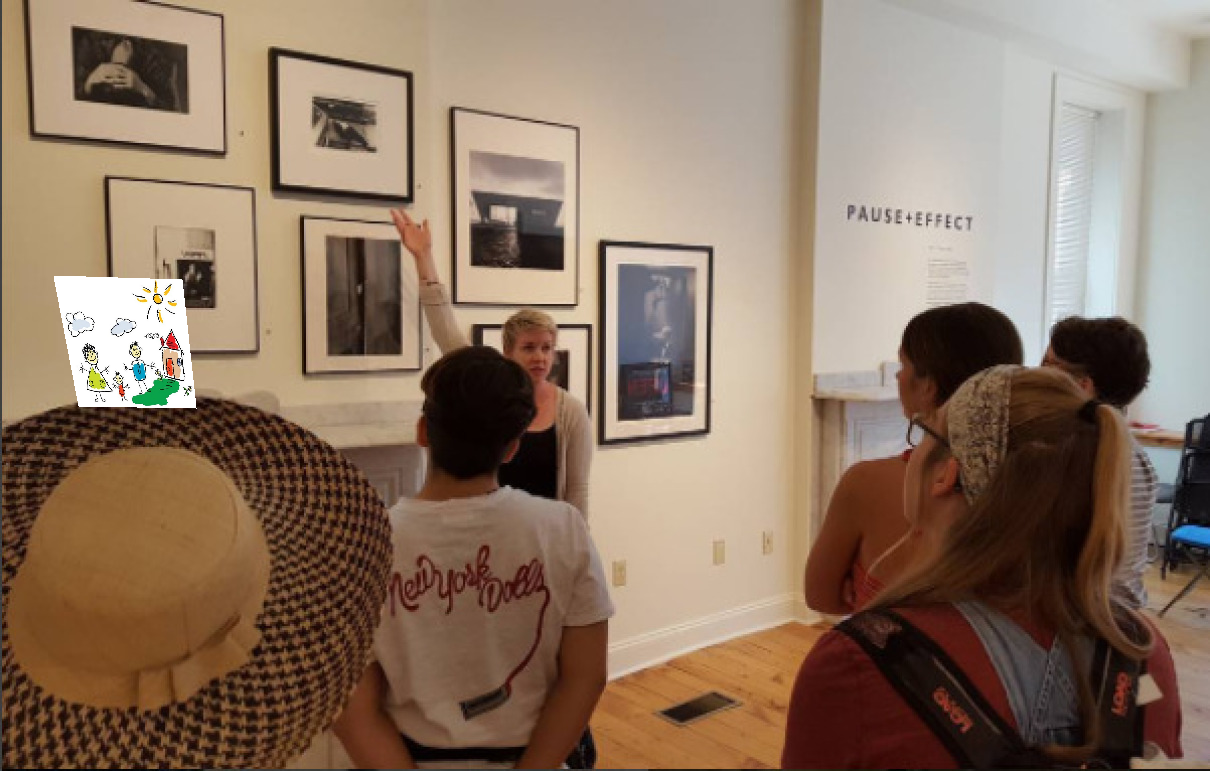
\includegraphics[width = \textwidth]{./code/outputs/prob4.png}
  \caption{Problem 4}
  \label{fig:4}
\end{figure}

\solution{5}
The result figure is shown as figure [\ref{fig:5}].
\begin{figure}[htbp]
  \centering
  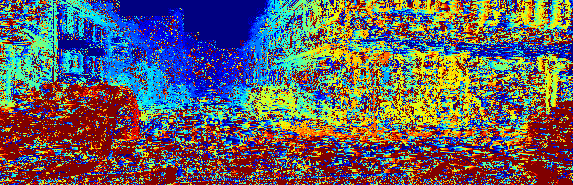
\includegraphics[width = \textwidth]{./code/outputs/prob5.png}
  \caption{Problem 5}
  \label{fig:5}
\end{figure}
%%%%%%%%%% Important, you must edit and complete the informational
%%%%%%%%%% section below. If you discus/sed the problem set with no
%%%%%%%%%% one, edit it to say no discussions or external resources.
\info

This problem set took approximately 16.5 hours of effort.

% Note that you might have to escape some special symbols in URLS like \_
I also got hints from the following sources:
\begin{itemize}
\item Wikipedia article on ordinary least squares at https://en.wikipedia.org/wiki/Ordinary\_least\_squares
\end{itemize}

\end{document}
